
\chapter{Descripción de la investigación}

\section{Título y definición del tema de investigación}

El título propuesto para el trabajo es "PROTOTIPO DE USO DE MACHINE LEARNING APLICADA EN EL ANÁLISIS DE LOS FACTORES QUE INFLUYEN EN LA CALIDAD DEL AIRE EN LA CIUDAD DE BOGOTÁ".


\section{Estudio del problema de investigación}

\subsection{Planteamiento del problema}

El número de datos ambientales recolectados por las estaciones de monitoreo en la ciudad de Bogotá a cargo de La Red de Monitoreo de Calidad del Aire de Bogotá - RMCAB que hace parte de la Subdirección de Calidad del Aire, Auditiva y Visual de la Secretaría Distrital de Ambiente y está conformada por catorce (14) estaciones de las cuales trece (13) son fijas y una (1) estación móvil y cuyas mediciones son realizadas en tiempo real y en periodos  cortos entre una medición y otra, garantizan la precisión de los indicadores de la calidad del aire, las concentraciones de material particulado (PM10 y PM2.5), la concentración de ozono (O3) , la concentración de dióxido de nitrógeno (NO2), la concentración de dióxido de azufre (SO2) y la concentración de monóxido de carbono (CO) en el aire, permitiéndonos conocer el comportamiento de la calidad del aire en las distintas zonas de la ciudad.[1]
Pero para registrar los cambios ocurridos, descubrir relaciones entre los datos y patrones en la dinámica de los fenómenos a través del volumen de datos obtenidos, exige que se usen herramientas informáticas para su almacenamiento y gestión que permitan tener un mecanismo eficiente de análisis de datos y extracción de información y conocimiento relevante para la toma de decisiones y la generación de alertas tempranas por medio de la predicción de comportamientos.
Es decir, es necesario contar con un modelo de gestión de datos para el análisis y extracción de información concreta que ayude, tanto a la toma de decisiones como a la construcción de mecanismos de alerta temprana, basados en predicción de eventos a partir del estudio de los datos históricos calculados a partir de estos.
Lo anterior se convierte en una oportunidad para la aplicación de técnicas de análisis de datos machine learning, el uso de datos masivos y sus técnicas analíticas para el diseño e implementación de políticas públicas que redunden en el beneficio de la sociedad.
Es por esto que las técnicas de machine learning han estado inmersos en muchos ámbitos de nuestra vida sin siquiera saberlo, Marketing y ventas son quizá las áreas de mayor aplicación en la actualidad, pero también se ve en otros ámbitos, como en los procesos de negocios, cuantificación y optimización del rendimiento personal, mejoramiento de la salud pública y un uso sorprendente es el de análisis de datos masivos para predecir la evolución de las epidemias y brotes de enfermedades. Integrando datos de historiales clínicos con análisis de datos de redes sociales pueden detectar brotes de enfermedades en tiempo real simplemente escuchando lo que la gente publica en sus perfiles públicos etc.
Todo esto nos lleva a cuestionarnos cómo los gobiernos llevan a cabo el aprovechamiento de los grandes volúmenes de información de sus datos para su gobernabilidad y toma de decisiones críticas, a la hora de invertir, ejecutar y proyectar soluciones en materia medioambiental, que si no son vistas desde una óptica propositiva no llegan a tener el impacto esperado al no generar las soluciones necesarias y esperadas.


\subsection{Formulación del problema}

¿La aplicación de machine learning en fuentes de datos abiertas de las diferentes entidades gubernamentales puede producir resultados específicos para la toma de decisiones en        el ámbito medioambiental de la ciudad de Bogotá?

\subsection{Sistematización del problema}

\begin{itemize}
	\item ¿Se pueden encontrar dataset de tipo público que ofrecen las entidades gubernamentales de la ciudad de Bogotá para la obtención de información relevante? 
	\item ¿Se pueden determinar las problemáticas de medio ambiente que suceden en la ciudad de Bogotá con la aplicación de machine learning sobre dataset de uso público? 
	\item ¿Qué tecnologías asociadas a machine learning se pueden adaptar mejor para el tratamiento de grandes volúmenes de datos ambientales? 
	\item ¿Se puede evaluar la eficacia del prototipo y determinar medidas de mejora para versiones posteriores? 
	\item ¿Es posible aplicar el enfoque machine learning a los datos ambientales referentes a la calidad del aire y resolver los problemas presentes en la contaminación del aire?
\end{itemize}

\section{Objetivos de la investigación}

\subsection{Objetivo general}

Diseñar un prototipo de machine learning que permita crear un modelo de predicción mediante la utilización de datos históricos asociados a la contaminación del aire de la ciudad de Bogotá haciendo uso de dataset públicos ofrecidos por las instituciones distritales.

\subsection{Objetivos específicos}

\begin{itemize}
	\item Identificar los dataset de las entidades estatales y nacionales que puedan ser usados para el desarrollo de nuestro prototipo como fuente de información para establecer las principales problemáticas del sector de medio ambiente en la ciudad de Bogotá.
	\item Identificar las fuentes de datos ambientales generados por estaciones de monitoreo ambiental que permitan mediante técnicas de inteligencia artificial el análisis predictivo de la calidad del aire.
	\item Realizar un análisis de los resultados obtenidos por parte del prototipo para determinar su nivel de eficacia.
	\item Determinar los modelos predictivos que puedan ser usados con mayor eficacia en la predicción de los niveles de crecimiento de los agentes contaminantes del aire en la ciudad.
	\item Caracterizar los modelos predictivos por su eficacia en la identificación de aumentos de agentes contaminantes.
	\item Determinar si es posible establecer una predicción del índice de los agentes contaminantes al año 2030.
\end{itemize}

\section{Justificación}

\subsection{Justificación práctica}

A lo largo de la última década se han visibilizado nuevas disciplinas en el campo tecnológico esto debido al crecimiento exponencial del uso de recursos tecnológicos en los diferentes ámbitos de nuestras vidas. A nivel mundial se ha dado la tendencia de automatización de procesos y análisis de datos, donde el objetivo es la identificación de patrones y tendencias en muchas diferentes fuentes de datos, una de las más destacada es el machine learning mediante el cual se puede explotar de forma más profunda las diferentes fuentes de datos para obtener la información más importante a la hora de tomar decisiones.
En Colombia desde el 17 de abril de 2018 se estableció la política de explotación de datos Big data en el documento CONPES 3920 la cual tiene como objetivo “La presente política tiene por objetivo aumentar el aprovechamiento de datos, mediante el desarrollo de las condiciones para que sean gestionados como activos para generar valor social y económico. En lo que se refiere a las actividades de las entidades públicas, esta generación de valor es entendida como la provisión de bienes públicos para brindar respuestas efectivas y útiles frente a las necesidades sociales” [2], de acuerdo a esto se busca crear un prototipo o modelo que permita realizar la aplicación de machine learning   en las diferentes fuentes de datos abiertas ofrecidas por las entidades estatales y nacionales, las que más tienen avances en la preparación de sus datos son: Red de Monitoreo de Calidad del Aire de Bogotá – RMCAB.[1]
Esta información sumada a la problemática de La calidad del aire es uno de los factores de importancia en la determinación del índice de calidad de vida de un centro urbano. 
Una ciudad con buena calidad del aire es preferible para vivir y más atractiva para las inversiones al ser comparada con otras ciudades con condiciones similares de ingreso, acceso a bienes y servicios y oportunidades de empleo, pero con aire contaminado. Un aire de baja calidad es aquel que produce una evidencia perceptible o medida de poco bienestar, v.g.: visibilidad reducida, suciedad en edificaciones, afectaciones a la naturaleza o perjuicios sobre la salud. En centros urbanos con altas concentraciones de población y la alta ocurrencia de procesos productivos, la afectación a la salud resulta ser la consecuencia más importante de la contaminación del aire. [1]
Es por lo que un análisis utilizando técnicas IA de machine learning permitirá catalizar la información obtenida y generar índices de valor para la toma de decisiones en materia ambiental a fin de solventar la problemática actual.
 

\section{Hipótesis del trabajo}

El adecuado aprovechamiento de los datos recolectados por las estaciones de monitoreo llevados a cabo por la Red de monitoreo de la calidad del aire de la ciudad de Bogotá permite tener un conocimiento en tiempo real de lo que está sucediendo con el aire en la ciudad, es por ello que contar con las herramientas y los métodos adecuados de análisis que permitan tomar acciones preventivas a través del aprendizaje automático la IA descarta por sí misma las acciones más arriesgadas y aquellas que pueden poner en riesgo el desarrollo normal de los factores económicos, sociales y culturales de la ciudad.
Debido a esto y con base en el planteamiento del problema definido antes, se define la siguiente hipótesis: “Con la elaboración de un prototipo usando tecnologías de machine learning aplicado en el análisis de los factores que influyen en la calidad del aire, se aportará favorablemente en el mejoramiento de la calidad del aire de la ciudad a través de resultados de información que permitirán tener herramientas más confiables para la toma de decisiones de índole medioambiental.”

\section{Marco referencial}

\subsection{Marco teórico}

El enfoque que la ciencia de los datos puede aportar al beneficio de una sociedad mejor adaptada a los cambios climáticos siempre redundarán en mejor entendimiento de entorno y su aprovechamiento de forma ecológicamente responsable.
En el artículo La contaminación del aire: su repercusión como problema de salud define a la contaminación del aire como cualquier modificación indeseable del ambiente, causada por la introducción a este de agentes físicos, químicos o biológicos (contaminantes) en cantidades superiores a las naturales, que resulta nociva para la salud humana, daña los recursos naturales o altera el equilibrio ecológico. \cite{ROMEROPLACERES2006}

En el artículo efectos de la contaminación atmosférica sobre la salud una introducción. Nos deja ver de una forma categórica como los retos relacionados con la exposición a la contaminación atmosférica son diversos, los más estudiados son aquellos que se producen a corto plazo es decir con el período de unos pocos días habitualmente menos de una semana después de la exposición a estos efectos, aunque mantiene una gran duración tanto de la gravedad de sus consecuencias como la población arriesgo afectada, además deben estar relacionados por el principio de coherencia; Por ejemplo si el hallazgo principal genera un aumento de la mortalidad total o por una causa específica se debería esperar necesariamente salvo que todos los que mueren en exceso ya estén hospitalizados. 
Aunque los niveles actuales de contaminación atmosférica en los países del Mundo occidental pueden, en general, considerarse moderados, la preocupación acerca de sus posibles efectos en la salud, de las personas persisten por un lado en los últimos años, un número importante de estudios realizados en distintas ciudades ha encontrado que aún por debajo de los niveles de calidad del aire considerados como seguros, los incrementos de los niveles de la contaminación atmosférica se asocian con efectos nocivos sobre la salud.\cite{BALLESTERDIEZ1999}

En el artículo Efectos de la calidad del aire sobre la salud nos presenta de forma caracterizada cuales son esos agentes contaminantes y como el deterioro de la calidad del aire, ya sea por causas antropogénicas o naturales, tiene efectos negativos sobre la salud humana y los ecosistemas y a escala global contribuye al cambio climático. Las causas antropogénicas son las que hoy tienen más efectos negativos y han aumentado en las últimas décadas. Aportan a la atmósfera contaminantes como: dióxido de carbono (CO2), monóxido de carbono (CO), dióxido de azufre (SO2), monóxido de nitrógeno (NO), dióxido de nitrógeno (NO2), ozono (O3) troposférico, amoníaco (NH3), ácido sulfhídrico (H2S) y partículas de medidas y composición muy diversa (metales, compuestos inorgánicos, compuestos orgánicos persistentes, compuestos orgánicos volátiles). En las partículas, es su tamaño lo que las hace más o menos perjudiciales; las más peligrosas son las de medida respirable inferior a 10$\mu$g, que pasan fácilmente al aparato respiratorio, y las de tamaño inferior a 2,5$\mu$g, que del alvéolo pulmonar pasan a la sangre y pueden afectar a todos los órganos, tejidos y células del organismo.\cite{MARTIVALLS2017511}

En el artículo análisis del estado de la calidad del aire en Bogotá advierte como los niveles de precipitación atmosférica no son tan relevantes a la hora de mitigar los efectos de la contaminación.
El análisis de los datos de calidad del aire en conjunto con la información meteorológica permite establecer, que la velocidad del viento, es el parámetro más influyente por encima de la intensidad de precipitación; en los niveles de contaminación por material particulado percibidos en la ciudad de Bogotá. \cite{GAITAN2007} 

En el artículo Contaminación del aire y vulnerabilidad de individuos expuestos: un caso de estudio para el centro de Medellín nos deja ver cómo trabajar en el interior reduce la vulnerabilidad de individuos que reportan un síntoma leve, pero aumenta la vulnerabilidad de quienes reportan una enfermedad. La persistencia en la relevancia de los meses trabajando en la zona manifiesta una mayor relevancia de la persistencia en la exposición (meses) que de la intensidad en la exposición (horas). Además, individuos con pago tienden a ser vulnerables cuando se exponen una mayor cantidad de horas diarias en la zona, mientras los individuos sin pago tienen mayor vulnerabilidad asociada a la cantidad de meses que trabajan en la zona. \cite{GAVIRIAG2012}

En el artículo aplicación de métodos de interpolación y modelamiento geoestadístico y la evaluación de la calidad del aire en Bogotá D.C. Nos deja ver que tomando en cuenta la muestra tomada para el análisis de las variables seleccionadas concentración de ozono y material particulado pm10 en la zona urbana de Bogotá, se tiene que el método que mejor se comporta de los métodos utilizados, es el Kriging ordinario que proporcionan resultados más satisfactorios al tener errores de predicción más reducidos y un error medio cuadrático menor. Con la aplicación de la validación Cruzada además si aumenta el número de estaciones de monitoreo se producirán aún mejores resultados por este método.\cite{RODRIGUEZ2015}

En el artículo Machine Learning and Deep Learning Applications-A Vision vislumbra el amplio panorama en el que la inteligencia artificial puede ser aplicada, sus usos y metodologías que, para el enfoque de la investigación planteada, presenta una solución al caracterizar de forma rigurosa el ámbito descriptivo de los pronósticos y su eficacia probada en aprendizaje automático a la hora de predecir eventos.\cite{SHARMA2021}

En el artículo Multivariate Adaptative Regression Splines (MARS), una alternativa para el análisis de series de tiempoMultivariate Adaptive Regression Splines (MARS), an alternative for the analysis of time series, se presenta como una alternativa para la automatización de los aspectos de modelación de la regresión clásica, seleccionando las variables predictoras, estimando los valores perdidos, transformando variables, detectando interacciones, contrastando y asegurando la correcta construcción del modelo, y permitiendo resultados más exactos y completos, permitiendo configurar modelos hipotéticos y escenarios de carácter predictivos tomando en cuenta los factores estructurales que pudieran estar influyendo sobre los datasets evaluados.\cite{VANEGAS2017235}

En el artículo El análisis de series temporales: situación y perspectivas, presenta los modelos más utilizados en el análisis de series temporales, sus aplicaciones más importantes y algunas de las lineas abiertas de investigación. Se presentan en primer lugar los análisis descriptivos que se utilizaron extensamente hasta la segunda mitad del siglo XX para representar series temporales. Estos modelos fueron sustituidos por los modelos ARIMA y los modelos en el espacio de los estados, que han alcanzado a finales del siglo XX una posición central en las aplicaciones y pueden considerarse ya como los modelos clásicos de series. En la última parte del siglo XX comenzó el desarrollo de los modelos no lineales y no parámetricos, que han permitido la extensión del análisis de series a situaciones donde los modelos clásicos no resultan apropiados. \cite{DPSSANCHEZDERIVERA}

En el artículo Análisis de series de tiempo univariante aplicando metodología de Box-Jenkins para la predicción de ozono en la ciudad de Cali, Colombia muestra como mediante la modelación para la predicción a corto plazo de la concentración de ozono troposférico en la zona urbana de la ciudad de Cali, Colombia, mediante el análisis univariante de series de tiempo, permite la predicción del incremento de valores de concentración de ozono  hasta con 8 horas de anticipación. \cite{JARAMILLOAYERBE2007}

En la tesis Pronóstico de la calidad del aire en el área metropolitana de la Ciudad de México a través del análisis de las series de tiempo de los componentes del IMECA, nos muestra los distintos modelos que pueden ser aplicados, para el pronóstico de índices de la calidad del aire tomando como parámetros iniciales mediciones realizadas en series de tiempo en largos periodos, de igual manera concluyen que estos pronósticos, llevan una tendencia  a su efectividad en un plazo más corto. 
\cite{MLCECILIA2011} 

\subsection{Marco conceptual}

\subsubsection{Ciencia de los datos}

La ciencia de datos es el cuarto paradigma de la ciencia, después del experimento, la teoría y ciencias computacionales, abreviado como ciencia de datos, se refiere a la realización del análisis de datos como una ciencia empírica, aprendiendo directamente a partir de los datos mismos. Esto puede tomar la forma de recopilación de datos seguida de un análisis abierto sin preconcebidas hipótesis (a veces denominada descubrimiento o exploración de datos). El segundo método empírico se refiere a la formulación de una hipótesis, la recopilación de datos nuevos o preexistentes, para abordar la hipótesis, y la confirmación analítica o negación de la hipótesis (o la determinación de que se requiere información o estudio adicional). En ambos métodos, las conclusiones se basan en los datos. 

En muchos proyectos de ciencia de datos, los datos originales son examinados primero, lo que informa una hipótesis, que luego se investiga. Como en cualquier ciencia experimental, el resultado
Podría ser que la hipótesis original en sí necesita ser reformulada. 

El concepto clave es que la ciencia de datos es una ciencia empírica, realizando el proceso científico directamente sobre los datos. Hay que tener en cuenta que la hipótesis puede ser por una necesidad, o puede ser la reafirmación de una necesidad en términos de una hipótesis técnica.
La ciencia de datos es la extracción de conocimiento útil directamente de los datos a través de un proceso de descubrimiento, o de formulación de hipótesis y prueba de hipótesis.

La ciencia de datos está estrechamente vinculada al análisis de Big Data y se refiere a la gestión y ejecución de los procesos de datos de un extremo a otro, incluidos los comportamientos de los componentes del sistema de datos. Como tal, la ciencia de datos
incluye toda la analítica, pero la analítica no incluye toda la ciencia de datos. La ciencia de datos contiene diferentes enfoques para aprovechar los datos para resolver las necesidades de la misión. Si bien el término ciencia de datos puede entenderse como las actividades en cualquier canal de análisis que produce conocimiento a partir de datos, el término se usa típicamente en el contexto de Big Data.

\subsubsection{Componente ambiental}

Las dinámicas de los recursos naturales y el medio ambiente generan una cantidad de datos considerable, los cuales son medidos, almacenados y analizados. Tratar estos datos exige de un gran esfuerzo, pero pueden contribuir de manera significativa a la generación de conocimiento, de patrones de comportamiento, de alertas de prevención y de políticas ambientales para apoyo a la toma de decisiones.
Dentro de las variables medioambientales que se pueden monitorear y que generan datos de forma continua se encuentran las de la medición de la calidad del aire.
El aire es una mezcla de gases que constituye la atmósfera que envuelve la tierra y es un factor indispensable para la vida. La presencia en el aire de una sustancia extraña o una variación significativa en la proporción de sus constituyentes susceptibles de provocar un efecto perjudicial, de origen antrópico, se conoce como contaminación atmosférica (Arnedo, et. al., 2005) fenómeno que se ha asociado con efectos nocivos para el entorno en general y para la salud humana en particular.

\subsubsection{Calidad del aire}

La quema de combustibles de biomasa y carbón para la preparación de alimentos, el uso de combustibles fósiles para la movilización de vehículos y para la producción industrial y el desarrollo exponencial de compuestos químicos, se identifican como algunas de las causas de la contaminación del aire (Enkerlin, Cano, Garza y Vogel. 1997).
Dentro de todos los contaminantes que existen en la atmósfera, se identificaron 5 contaminantes criterio que afectan a la salud inmediatamente desde su inhalación: monóxido de carbono (CO), dióxido de azufre (SO2), dióxido de nitrógeno (NO2), ozono troposférico (O3) y material particulado con diámetro aerodinámico menor a 10 µm (PM10). Además de éstos, se incluye al CO2 (dióxido de carbono) por su aporte al efecto invernadero.

En los últimos diez años, las partículas totales en suspensión más importantes son las conocidas como PM10 y PM2.5, respectivamente. La razón fundamental de esta especificación se debe a que las partículas más pequeñas son más peligrosas para la salud de los seres humanos porque son capaces de alcanzar la zona inferior de los pulmones (OPS, 2005a). A continuación, se listan algunos de los efectos más importantes en la salud (OPS, 2005b) para los contaminantes  como son material particulado, óxidos de azufre, óxidos de nitrógeno y ozono.

\begin{itemize}
	\item Dióxido de azufre (SO2). La exposición a SO2 puede disminuir la función pulmonar, agravar enfermedades respiratorias preexistentes (especialmente bronquitis) y reducir la habilidad de los pulmones para liberar partículas extrañas.
	\item Dióxido de nitrógeno (NO2). El monóxido de nitrógeno (NO) es relativamente inofensivo, sin embargo, el NO2 puede causar problemas respiratorios principalmente en asmáticos y niños.
	\item Ozono (O3). Cabe anotar que el ozono producido naturalmente en la estratosfera es beneficioso porque protege a la tierra y sus habitantes de la nociva radiación ultravioleta del sol.
	\item Material particulado (MP). Son las partículas sólidas o líquidas suspendidas en el aire, tienen una composición química diversa y su tamaño varía de 0.005 a 100 mm de diámetro aerodinámico; sus
	fuentes principales son la quema incompleta del combustible para motores diésel y los combustibles sólidos, como la madera y el carbón, también se puede producir por la condensación de vapores ácidos y compuestos orgánicos semi-volátiles, mediante una serie de complejas reacciones del NO2 y SO2 en la atmósfera que finalmente forman sales de nitratos y sulfatos.
\end{itemize}

Las partículas que más afectan la salud son aquellas con diámetro aerodinámico menor de 10 mm (PM10) y, más aún, aquéllas con diámetro aerodinámico menor de 2,5 mm (MP2.5).

\subsubsection{Aire y contaminación}

El aire es una mezcla de gases que constituye la atmósfera que envuelve la tierra y es un factor indispensable para la vida. 
La presencia en el aire de una sustancia extraña o una variación significativa en la proporción de sus constituyentes susceptibles de provocar un efecto perjudicial, de origen antrópico, se conoce como contaminación atmosférica (Arnedo, et. al., 2005) fenómeno que se ha asociado con efectos nocivos para el entorno en general y para la salud humana en particular.

\subsubsection{Red de monitoreo de calidad del aire de Bogotá}

El Distrito Capital cuenta con la Red de Monitoreo de Calidad del Aire de Bogotá – RMCAB, que permite recolectar información sobre la concentración de contaminantes de origen antropogénico y natural y el comportamiento de las variables meteorológicas que regulan la distribución de los mismos en la atmósfera bogotana.
Los datos recolectados en distintos sitios de la ciudad se reciben en una estación central donde se someten a un proceso de validación final y posterior análisis con el fin de evaluar el cumplimiento de los estándares de calidad de aire en Bogotá dados por la Resolución 610 del 24 de marzo de 2010 expedida por el entonces Ministerio de Ambiente, Vivienda y Desarrollo Territorial (MAVDT). Además resulta información base para la definición de las políticas de control de la contaminación y de la gestión ambiental.
Para el año 2019 la RMCAB estaba conformada por catorce (14) estaciones de monitoreo de las cuales doce (12) son fijas, una (1) meteorológica y una (1) móvil. Están ubicadas en sitios estratégicos de la ciudad, dotadas con equipos automáticos que permiten realizar un monitoreo continuo de las concentraciones de contaminantes criterio: material particulado (PM10, PM2.5), y gases contaminantes (SO2, NO2, CO, O3), así como de las variables meteorológicas de Precipitación, Velocidad y Dirección del Viento, Temperatura, Radiación Solar, Humedad Relativa y Presión Barométrica.
Los métodos de medición utilizados por la RMCAB se encuentran descritos en el CFR (Code of Federal Regulations) Título 40 que están aprobados por la Environmental Protection Agency (EPA) de Estados Unidos (U.S. Governement Printing Office, 2014).
El comportamiento del contaminante PM10 se puede observar en el gráfico de boxplot presentado en la Figura 2, el cual se ha usado históricamente como referencia para definir los niveles de contaminación y definir políticas de control ambiental.

\begin{figure}[h]
	\centering
	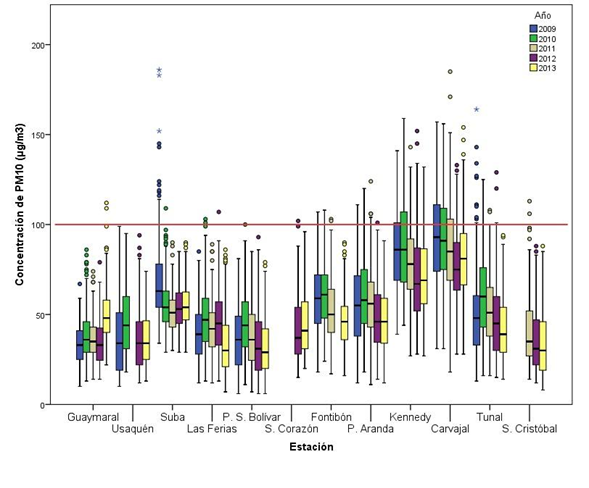
\includegraphics[scale=0.8]{images/BoxPlot.png}
	\caption{Gráfico boxplot}
\end{figure}

Se puede observar que en términos generales existe una tendencia a la reducción progresiva en los niveles de concentración en los últimos años y para la mayoría de estaciones. Sin embargo y comparando los dos últimos años 2012 y 2013, se puede apreciar que  para las estaciones de San Cristóbal, Tunal, Fontibón, Parque Simón Bolívar y Las Ferias existe una reducción en los niveles de concentración; mientras que otras estaciones como Puente Aranda, Suba y Usaquén han permanecido constantes.
Por su parte las estaciones Carvajal, Kennedy, Sagrado Corazón y Guaymaral presentaron aumentos en las concentraciones de 2013 en comparación a 2012 y además para el caso de Carvajal y Kennedy resultan los sitios de monitoreo en la ciudad con los mayores niveles de concentración con valores promedio de 81 y 71 µg/m3 y también en donde mayores excedencias a la norma diaria existen.

\subsubsection{Información de contaminantes}

\boldmath{$SO_2$} 
El dióxido de azufre es un gas incoloro y no inflamable, de olor fuerte e irritante. Su vida media en la atmósfera es corta de unos 2 a 4 días, y casi la mitad de las emisiones vuelven a depositarse en la superficie, mientras que el resto se transforma en iones sulfato (SO42-). Se trata de una sustancia reductora, que con el tiempo y en contacto con el aire y la humedad, se convierte en trióxido de azufre. Es soluble en agua, formando una disolución ácida, y aún siendo inestable en estas condiciones, es capaz de formar sales como los sulfitos y bisulfitos.

\textbf{PM10} 
Las PM10 se pueden definir como aquellas partículas sólidas o líquidas de polvo, cenizas, hollín, partículas metálicas, cemento o polen, dispersas en la atmósfera, y cuyo diámetro varía entre 2,5 y 10 µm (1 micrómetro corresponde la milésima parte de 1 milímetro).

\textbf{PM2.5} 
Son partículas que tienen diámetro aerodinámico inferior o igual a los 2,5 micrómetros, es decir, son 100 veces más delgadas que un cabello humano.
Además, el tamaño no es la única diferencia. Cada tipo de partículas está compuesto de diferente material y puede provenir de diferentes fuentes. En el caso de las PM2.5, su origen está principalmente en fuentes de carácter antropogénico como las emisiones de los vehículos diésel.


El monóxido de carbono, cuya fórmula química es CO, es un gas incoloro y altamente tóxico. Puede causar la muerte cuando se respira en niveles elevados. Se produce por la combustión deficiente de sustancias como gas, gasolina, queroseno, carbón, petróleo, tabaco o madera. Las chimeneas, las calderas, los calentadores de agua o calefactores y los aparatos domésticos que queman combustible, como las estufas u hornillas de la cocina o los calentadores a queroseno, también pueden producirlo si no están funcionando bien. Los vehículos con el motor encendido también lo expulsan. Grandes cantidades de CO se forman como subproducto durante los procesos oxidativos para la producción de productos químicos, lo que hace necesaria la purificación de los gases residuales. 

\textbf{Ozono}
El ozono es un gas incoloro e inestable de tres átomos de oxígeno (su fórmula química es O3), además, es un oxidante fuerte, muy fácil de producir pero a la vez muy frágil y fácil de destruir. Este gas reacciona fácilmente con muchos compuestos químicos y es explosivo en pequeñas cantidades. En 1840 el gas fue bautizado como "ozono" (el olor) por el químico Christian Friedrich Schönbein, quien descubrió que esta sustancia se formaba durante descargas eléctricas. Muy pronto se descubrió que el ozono era un componente natural del aire. Se caracteriza por su olor peculiar, el cual puede ser detectado durante los episodios de tormentas eléctricas y en las proximidades de equipos eléctricos. Las descargas eléctricas son generalmente usadas en la producción de ozono para procesos industriales, tales como, la purificación de agua y aire y el blanqueamiento de textiles y productos alimenticios.

\textbf{Dióxido de nitrógeno}
El dióxido de nitrógeno u óxido de nitrógeno (IV)2 (NO2), es un compuesto químico formado por los elementos nitrógeno y oxígeno, uno de los principales contaminantes entre los varios óxidos de nitrógeno.
El dióxido de nitrógeno es de color marrón-amarillento. Se forma como subproducto en los procesos de combustión a altas temperaturas, como en los vehículos motorizados y las plantas eléctricas. Por ello es un contaminante frecuente en zonas urbanas.

\textbf{Benceno}
El benceno es un hidrocarburo aromático de fórmula molecular C6H6, (originariamente a él y sus derivados se le denominaban compuestos aromáticos debido a la forma característica que poseen) también es conocido como benzol. En el benceno cada átomo de carbono ocupa el vértice de un hexágono regular, aparentemente tres de las cuatro valencias de los átomos de carbono se utilizan para unir átomos de carbono contiguos entre sí, y la cuarta valencia con un átomo de hidrógeno. Según las teorías modernas sobre los enlaces químicos, tres de los cuatro electrones de la capa de valencia del átomo de carbono se utilizan directamente para formar los enlaces covalentes típicos (2C-C y C-H) y el cuarto se comparte con los de los otros cinco átomos de carbono, obteniéndose lo que se denomina "la nube (pi)" que contiene en diversos orbitales los seis electrones. El benceno es un líquido incoloro y muy inflamable de aroma dulce (que debe manejarse con sumo cuidado debido a su carácter cancerígeno), con un punto de ebullición relativamente alto.

\subsubsection{Niveles máximos permisibles de contaminantes criterio en el aire}

\textbf{\textit{Resolución 2254 de 2017}}

\textit{"Artículo 2°. Niveles máximos permisibles de contaminantes criterio. En la Tabla número 1 se establecen los niveles máximos permisibles a condiciones de referencia para contaminantes criterio que regirán a partir del primero de enero del año 2018:"}

\begin{table}[h!]
	\begin{center}
		\begin{tabular}{| c | c | c |}
			\hline
			\rowcolor{lightgray}Contaminante 	& Nivel máximo permisible ($ \mu g/m^3 $) 	& Tiempo de exposición	\\ \hline
			PM10			& 50 		& Anual		\\
			  				& 100 		& 24 horas	\\ \hline
			PM2.5 			& 25 		& Anual 	\\
				 			& 50 		& 24 horas	\\ \hline
 			$ SO_2 $		& 50 		& 24 horas 	\\
 							& 100 		& 1 hora	\\ \hline
 			$ NO_2 $		& 60 		& Anual 	\\
 							& 200 		& 1 hora	\\ \hline
 			$ O_3 $			& 100 		& 8 horas 	\\ \hline
 			$ CO $			& 5000 		& 8 horas 	\\
 							& 35000 	& 1 hora	\\ \hline
		\end{tabular}
		\caption{Niveles máximos permisibles de contaminantes criterio en el aire}
	\end{center}
\end{table}

\textit{"Parágrafo 1°. A partir del 1° de julio de 2018, los niveles máximos permisibles de PM10 y PM2.5 para un tiempo de exposición 24 horas serán de 75 µg/m3 y 37 µg/m3 respectivamente."}

\textit{"Parágrafo 2°. Para verificar el cumplimiento de los niveles máximos permisibles establecidos en la Tabla número 1, la concentración de los contaminantes del aire deberá evaluarse por cada punto de monitoreo. El promedio de concentraciones de diferentes puntos de monitoreo no será válido para evaluar el cumplimiento de dichos niveles."}

\textit{"Parágrafo 3°. Las autoridades ambientales competentes deben realizar las mediciones de los contaminantes criterio establecidos en el presente artículo, de acuerdo con los procedimientos, frecuencias y metodologías establecidas en el Protocolo para el Monitoreo y Seguimiento de la Calidad del Aire."}

\textit{"Parágrafo 4°. Con el objetivo de identificar fuentes de emisión, soportar investigaciones en salud ambiental y sus efectos sobre el clima, las autoridades ambientales competentes podrán monitorear las concentraciones en la atmósfera de carbono negro y otros contaminantes climáticos. Los resultados que se generen por parte de las autoridades ambientales deberán reportarse al Subsistema de Información sobre Calidad del Aire (SISAIRE)."}

\textit{"Artículo 3°. Niveles Máximos Permisibles a 2030. En la Tabla número 2 se establecen los niveles máximos permisibles a condiciones de referencia para contaminantes criterio que regirán a partir del 1° de enero del año 2030"}

\begin{table}[h!]
	\begin{center}
		\begin{tabular}{| c | c | c |}
			\hline
			\rowcolor{lightgray}
			Contaminante 	& Nivel máximo permisible ($ \mu g/m^3 $) 	& Tiempo de exposición	\\ \hline
			PM10			& 30 		& Anual		\\ \hline
			PM2.5 			& 15 		& Anual 	\\ \hline
			$ SO_2 $		& 20 		& 24 horas 	\\ \hline
			$ NO_2 $		& 40 		& Anual 	\\ \hline
		\end{tabular}
		\caption{Niveles máximos permisibles de contaminantes en el aire para el año 2030}
	\end{center}
\end{table}


\textit{"Lo dispuesto en los parágrafos 1° y 2° del artículo 2° será aplicable al presente artículo."}

\textit{"Parágrafo. Para los contaminantes y tiempos de exposición que no se encuentren en la Tabla número 2 se mantendrán los establecidos en la Tabla No. 1 de la presente resolución."}

\textit{"Artículo 4°. Niveles máximos permisibles de contaminantes tóxicos del aire. En la Tabla número 3 se establecen los niveles máximos permisibles a condiciones de referencia para contaminantes tóxicos del aire, teniendo en cuenta sus efectos adversos en la salud humana y el ambiente. Estos niveles regirán a partir del 1° de enero de 2018."}

\begin{table}[h]
	\begin{center}
		\begin{tabular}{| p{4cm} | c | c |}
			\hline
			\rowcolor{lightgray}
			Contaminantes tóxicos 			& Nivel máximo permisible ($ \mu g/m^3 $) 	& Tiempo de exposición	\\ \hline
			Plomo y sus compuestos			& 0.5 		& Anual		\\ \hline
			Cadmio							& 0.005 	& Anual 	\\ \hline
			Benceno							& 5 		& Anual		\\ \hline
			Mercurio inorgánico(vapores)	& 1 		& Anual		\\ \hline
			Tolueno							& 260 		& 1 Semana 	\\ 
											& 1000 		& 30 Minutos\\ \hline
			Níquel y sus compuestos			& 260 		& Anual 	\\ \hline
			Hidrocarburos aromáticos Policíclicos expresados como benzo (a) pireno	& 0.001	& Anual 	\\ \hline
		\end{tabular}
		\caption{Niveles máximos permisibles de contaminantes tóxicos en el aire}
	\end{center}
\end{table}

\subsubsection{Machine Learning}

Pero, ¿qué es exactamente Machine Learning?. El Machine Learning es el diseño y estudio de las herramientas informáticas que utilizan la experiencia pasada para tomar decisiones futuras; es el estudio de programas que pueden aprender de los datos. El objetivo fundamental del Machine Learning es generalizar, o inducir una regla desconocida a partir de ejemplos donde esa regla es aplicada. El ejemplo más típico donde podemos ver el uso del Machine Learning es en el filtrado de los correos basura o spam. Mediante la observación de miles de correos electrónicos que han sido marcados previamente como basura, los filtros de spam aprenden a clasificar los mensajes nuevos. El Machine Learning combina conceptos y técnicas de diferentes áreas del conocimiento, como las matemáticas, estadísticas y las ciencias de la computación; por tal motivo, hay muchas maneras de aprender la disciplina.

\textbf{Tipos de machine learning}

El Machine Learning tiene una amplia gama de aplicaciones, incluyendo motores de búsqueda, diagnósticos médicos, detección de fraude en el uso de tarjetas de crédito, análisis del mercado de valores, clasificación de secuencias de ADN, reconocimiento del habla y del lenguaje escrito, juegos y robótica. Pero para poder abordar cada uno de estos temas es crucial en primer lugar distinguir los distintos tipos de problemas de Machine Learning con los que nos podemos encontrar.

\textbf{\textit{Aprendizaje supervisado}} En los problemas de aprendizaje supervisado se enseña o entrena al algoritmo a partir de datos que ya vienen etiquetados con la respuesta correcta. Cuanto mayor es el conjunto de datos más el algoritmo puede aprender sobre el tema. Una vez concluído el entrenamiento, se le brindan nuevos datos, ya sin las etiquetas de las respuestas correctas, y el algoritmo de aprendizaje utiliza la experiencia pasada que adquirió durante la etapa de entrenamiento para predecir un resultado. Esto es similar al método de aprendizaje que se utiliza en las escuelas, donde se nos enseñan problemas y las formas de resolverlos, para que luego podamos aplicar los mismos métodos en situaciones similares.

\textbf{\textit{Aprendizaje no supervisado}} En los problemas de aprendizaje no supervisado el algoritmo es entrenado usando un conjunto de datos que no tiene ninguna etiqueta; en este caso, nunca se le dice al algoritmo lo que representan los datos. La idea es que el algoritmo pueda encontrar por si solo patrones que ayuden a entender el conjunto de datos. El aprendizaje no supervisado es similar al método que utilizamos para aprender a hablar cuando somos bebes, en un principio escuchamos hablar a nuestros padres y no entendemos nada; pero a medida que vamos escuchando miles de conversaciones, nuestro cerebro comenzará a formar un modelo sobre cómo funciona el lenguaje y comenzaremos a reconocer patrones y a esperar ciertos sonidos.


\textbf{\textit{Aprendizaje por refuerzo}} En los problemas de aprendizaje por refuerzo, el algoritmo aprende observando el mundo que le rodea. Su información de entrada es el feedback o retroalimentación que obtiene del mundo exterior como respuesta a sus acciones. Por lo tanto, el sistema aprende a base de ensayo-error. Un buen ejemplo de este tipo de aprendizaje lo podemos encontrar en los juegos, donde vamos probando nuevas estrategias y vamos seleccionando y perfeccionando aquellas que nos ayudan a ganar el juego. A medida que vamos adquiriendo más practica, el efecto acumulativo del refuerzo a nuestras acciones victoriosas terminará creando una estrategia ganadora.

\textbf{\textit{Sobreajuste}} Como mencionamos cuando definimos al Machine Learning, la idea fundamental es encontrar patrones que podamos generalizar para luego poder aplicar esta generalización sobre los casos que todavía no hemos observado y realizar predicciones. Pero también puede ocurrir que durante el entrenamiento solo descubramos casualidades en los datos que se parecen a patrones interesantes, pero que no generalicen. Esto es lo que se conoce con el nombre de sobreajuste o sobreentrenamiento.

El sobreajuste es la tendencia que tienen la mayoría de los algoritmos de Machine Learning a ajustarse a unas características muy específicas de los datos de entrenamiento que no tienen relación causal con la función objetivo que estamos buscando para generalizar. El ejemplo más extremo de un modelo sobreajustado es un modelo que solo memoriza las respuestas correctas; este modelo al ser utilizado con datos que nunca antes ha visto va a tener un rendimiento azaroso, ya que nunca logró generalizar un patrón para predecir.

\textbf{\textit{Como evitar el sobreajuste}}
Como mencionamos anteriormente, todos los modelos de Machine Learning tienen tendencia al sobreajuste; es por esto que debemos aprender a convivir con el mismo y tratar de tomar medidas preventivas para reducirlo lo más posible. Las dos principales estrategias para lidiar son el sobreajuste son: la retención de datos y la validación cruzada.

En el primer caso, la idea es dividir nuestro conjunto de datos, en uno o varios conjuntos de entrenamiento y otro/s conjuntos de evaluación. Es decir, que no le vamos a pasar todos nuestros datos al algoritmo durante el entrenamiento, sino que vamos a retener una parte de los datos de entrenamiento para realizar una evaluación de la efectividad del modelo. Con esto lo que buscamos es evitar que los mismos datos que usamos para entrenar sean los mismos que utilizamos para evaluar. De esta forma vamos a poder analizar con más precisión como el modelo se va comportando a medida que más lo vamos entrenando y poder detectar el punto crítico en el que el modelo deja de generalizar y comienza a sobreajustarse a los datos de entrenamiento.

La validación cruzada es un procedimiento más sofisticado que el anterior. En lugar de solo obtener una simple estimación de la efectividad de la generalización; la idea es realizar un análisis estadístico para obtener otras medidas del rendimiento estimado, como la media y la varianza, y así poder entender cómo se espera que el rendimiento varíe a través de los distintos conjuntos de datos. Esta variación es fundamental para la evaluación de la confianza en la estimación del rendimiento. La validación cruzada también hace un mejor uso de un conjunto de datos limitado; ya que a diferencia de la simple división de los datos en uno el entrenamiento y otro de evaluación; la validación cruzada calcula sus estimaciones sobre todo el conjunto de datos mediante la realización de múltiples divisiones e intercambios sistemáticos entre datos de entrenamiento y datos de evaluación.

\textbf{Pasos para construir un modelo de Machine Learning}

Construir un modelo de Machine Learning, no se reduce solo a utilizar un algoritmo de aprendizaje o utilizar una librería de Machine Learning; sino que es todo un proceso que suele involucrar los siguientes pasos:

Recolectar los datos. Podemos recolectar los datos desde muchas fuentes, podemos por ejemplo extraer los datos de un sitio web o obtener los datos utilizando una API o desde una base de datos. Podemos también utilizar otros dispositivos que recolectan los datos por nosotros; o utilizar datos que son de dominio público. ¡El número de opciones que tenemos para recolectar datos no tiene fin! Este paso parece obvio, pero es uno de los que más complicaciones trae y más tiempo consume.

Preprocesar los datos. Una vez que tenemos los datos, tenemos que asegurarnos que tiene el formato correcto para nutrir nuestro algoritmo de aprendizaje. Es prácticamente inevitable tener que realizar varias tareas de preprocesamiento antes de poder utilizar los datos. Igualmente, este punto suele ser mucho más sencillo que el paso anterior.

Explorar los datos. Una vez que ya tenemos los datos y están con el formato correcto, podemos realizar un pre análisis para corregir los casos de valores faltantes o intentar encontrar a simple vista algún patrón en los mismos que nos facilite la construcción del modelo. En esta etapa suelen ser de mucha utilidad las medidas estadísticas y los gráficos en 2 y 3 dimensiones para tener una idea visual de cómo se comportan nuestros datos. En este punto podemos detectar valores atípicos que debamos descartar; o encontrar las características que más influencia tienen para realizar una predicción.

Entrenar el algoritmo. Aquí es donde comenzamos a utilizar las técnicas de Machine Learning realmente. En esta etapa nutrimos al o los algoritmos de aprendizaje con los datos que venimos procesando en las etapas anteriores. La idea es que los algoritmos puedan extraer información útil de los datos que le pasamos para luego poder hacer predicciones.

Evaluar el algoritmo. En esta etapa ponemos a prueba la información o conocimiento que el algoritmo obtuvo del entrenamiento del paso anterior. Evaluamos que tan preciso es el algoritmo en sus predicciones y si no estamos muy conforme con su rendimiento, podemos volver a la etapa anterior y continuar entrenando el algoritmo cambiando algunos parámetros hasta lograr un rendimiento aceptable.

Utilizar el modelo. En esta última etapa, ya ponemos a nuestro modelo a enfrentarse al problema real. Aquí también podemos medir su rendimiento, lo que tal vez nos obligue a revisar todos los pasos anteriores.

\textbf{Librerías de Python para machine Learning}


Como siempre me gusta comentar, una de las grandes ventajas que ofrece Python sobre otros lenguajes de programación; es lo grande y prolifera que es la comunidad de desarrolladores que lo rodean; comunidad que ha contribuido con una gran variedad de librerías de primer nivel que extienden las funcionalidades del lenguaje. Para el caso de Machine Learning, las principales librerías que podemos utilizar son:

\textbf{\textit{SCIKIT-LEARN}} Es la principal librería que existe para trabajar con Machine Learning, incluye la implementación de un gran número de algoritmos de aprendizaje. La podemos utilizar para clasificaciones, extracción de características, regresiones, agrupaciones, reducción de dimensiones, selección de modelos, o preprocesamiento. Posee una API que es consistente en todos los modelos y se integra muy bien con el resto de los paquetes científicos que ofrece Python. Esta librería también nos facilita las tareas de evaluación, diagnóstico y validaciones cruzadas ya que nos proporciona varios métodos de fábrica para poder realizar estas tareas en forma muy simple.

\textbf{\textit{STATSMODELS}} Es otra gran librería que hace foco en modelos estadísticos y se utiliza principalmente para análisis predictivos y exploratorios. Al igual que Scikit-learn, también se integra muy bien con el resto de los paquetes científicos de Python. Si deseamos ajustar modelos lineales, hacer un análisis estadístico, o tal vez un poco de modelado predictivo, entonces Statsmodels es la librería ideal. Las pruebas estadísticas que ofrece son bastante amplias y abarcan tareas de validación para la mayoría de los casos.

\textbf{\textit{PYMC}} Es un módulo de Python que implementa modelos estadísticos bayesianos, incluyendo la cadena de Markov Monte Carlo(MCMC). pyMC ofrece funcionalidades para hacer el análisis bayesiano lo más simple posible. Incluye los modelos bayesianos, distribuciones estadísticas y herramientas de diagnóstico para la covarianza de los modelos. Si queremos realizar un análisis bayesiano esta es sin duda la librería a utilizar.

\textbf{\textit{NTLK}} Es la librería líder para el procesamiento del lenguaje natural o NLP por sus siglas en inglés. Proporciona interfaces fáciles de usar a más de 50 cuerpos y recursos léxicos, como WordNet, junto con un conjunto de bibliotecas de procesamiento de texto para la clasificación, tokenización, el etiquetado, el análisis y el razonamiento semántico.


Obviamente, aquí solo estoy listando unas pocas de las muchas librerías que existen en Python para trabajar con problemas de Machine Learning, los invito a realizar su propia investigación sobre el tema


\section{Aspectos metodológicos}

\subsection{Tipo de estudio}

La naturaleza de este trabajo es de tipo propositivo ya que se pretende proponer un patrón de aprendizaje para contrastar con otros patrones.

\subsection{Metodología de investigación}

Para la ejecución del proyecto se plantean cuatro ciclos, cada ciclo está asociado al proceso del desarrollo de los objetivos, estos son a su vez caracterizados por una serie de actividades. Los ciclos y actividades de la metodología se resumen a continuación.

\begin{table}[h]
	\begin{center}
		\begin{tabular}{| p{4cm} | p{4cm} | p{4cm} |}
			\hline
			\rowcolor{lightgray}
			Ciclo 			& Objeto asociado 	& Tiempo de exposición	\\ \hline
			
			Ciclo 1: Obtención, revisión y refinamiento del marco conceptual y preparación de fuentes de datos para el modelo.			
			& Identificar los data set de las entidades estatales y nacionales que puedan ser usados para el desarrollo de nuestro prototipo como fuente de información para establecer las principales problemáticas del sector de medio ambiente en la ciudad de Bogotá.
			Identificar las fuentes de datos ambientales generados por estaciones de monitoreo ambiental que permitan mediante técnicas de inteligencia artificial el análisis predictivo de la calidad del aire.
	 		& Extracción de los data sets de calidad del aire por hora de la localidad de Kennedy del 1 de enero de 2010 a 6 de abril de 2021.
	 		Análisis exploratorio de los datos.\\ \hline
	 		
			Ciclo 2: Estudio, evaluación y comparación de las metodologias de machine learning para el desarrollo de pronósticos, análisis predictivos de información climática.							& Determinar los modelos predictivos que puedan ser usados con mayor eficacia en la predicción de los niveles de crecimiento de los agentes contaminantes del aire en la ciudad.	
			& Realizar un estudio de los diferentes métodos de machine learning que permitan realizar un pronóstico más exacto.  	\\ \hline
			
			Ciclo 3: Diseño del modelo para análisis predictivo de datos de la calidad del aire							
			& Caracterizar los modelos predictivos por su eficacia en la identificación de aumentos de agentes contaminantes.		
			& Dividir la serie en conjuntos de entrenamiento y prueba. para poder comparar los resultados entre los modelos a probar.
			
			Realizar prueba de estacionaridad, toda vez es necesaria para la utilización del modelo VAR
			
			Transformación de la serie de entrenamiento de ser necesaria.
			
			Construir un modelo VAR sobre las series transformadas.
			
			Emplear la causalidad de Granger.
			
			Realizar un diagnóstico del modelo.		\\ \hline
			
			
			Ciclo 4: Construcción y validación del prototipo.
			& Determinar si es posible establecer una predicción del índice de los agentes contaminantes al año 2030.		
			& Realizar un pronóstico utilizando el modelo finalmente elegido.
			
			Realizar una transformación inversa del pronóstico a la escala original.
			
			Realizar una evaluación del pronóstico	\\ \hline

		\end{tabular}
		\caption{Ciclos de actividades}
	\end{center}
\end{table}

\subsection{Fuentes y técnicas para la recolección de información}

Las principales fuentes de información identificadas son los datos e indicadores publicados por por el observatorio ambiental de Bogotá, donde está la información clasificada por zonas rurales y urbanas, también por localidades; otra fuente identificada es la plataforma de datos abiertos de Bogotá donde se encuentra la categoría de ambiente y desarrollo sostenible y donde hay diferentes dataset que pueden llegar a ser útiles para el desarrollo del proyecto.